\documentclass[preprint,12pt]{elsarticle}
\usepackage{lmodern}
\input{glyphtounicode}
\pdfgentounicode=1
\usepackage{amsmath,amssymb,amsfonts,mathtools,amsthm,bm}
\usepackage{booktabs,graphicx,array,tabularx,placeins,float,url}
\usepackage[hidelinks]{hyperref}
\hypersetup{pdfauthor={Ali Eslami and Jiangbo Yu}}
\usepackage[protrusion=true,expansion=false]{microtype}
\graphicspath{{figures/}{./}}
\allowdisplaybreaks
\setlength{\emergencystretch}{3em}
\interdisplaylinepenalty=2500
\newtheorem{assumption}{Assumption}
\newtheorem{theorem}{Theorem}
\newtheorem{proposition}{Proposition}
\newtheorem{corollary}{Corollary}
\newtheorem{remark}{Remark}
\newtheorem{definition}{Definition}
\newcommand{\R}{\mathbb{R}}
% elsarticle includes the word ``Appendix'' in appendix-section references.
\newcommand{\appref}[1]{\ref{#1}}


\renewcommand{\thesection}{S\arabic{section}}
\numberwithin{equation}{section}
\renewcommand{\thetable}{S\arabic{table}}
\renewcommand{\thefigure}{S\arabic{figure}}
\newcommand{\papernumber}[1]{\csname papernumber@#1\endcsname}
% Cross-document numbers: ordinary definitions; no external auxiliary dependency.
\expandafter\def\csname papernumber@app:repair-cost\endcsname{Appendix~F}
\expandafter\def\csname papernumber@eq:benchmark-native\endcsname{8}
\expandafter\def\csname papernumber@eq:network-jacobian\endcsname{35}
\expandafter\def\csname papernumber@eq:new-exact-actuator-residuals\endcsname{Appendix~B.7}
\expandafter\def\csname papernumber@eq:new-mfd\endcsname{2}
\expandafter\def\csname papernumber@prop:network-localization\endcsname{4}
\expandafter\def\csname papernumber@prop:planned-handover\endcsname{3}
\expandafter\def\csname papernumber@prop:repair-execution\endcsname{2}
\expandafter\def\csname papernumber@prop:structure-plan\endcsname{1}
\expandafter\def\csname papernumber@sec:terminal-backup\endcsname{Appendix~F.1}
\expandafter\def\csname papernumber@thm:repair-grid\endcsname{3}

\begin{document}
\begin{frontmatter}
\title{Supplementary Evidence and Implementation Details\\
Formal Guarantees for Trustworthy Agent-Mediated Urban Perimeter Control}
\author{Ali Eslami and Jiangbo Yu}
\begin{abstract}
This companion preserves complete experiment settings, detailed results and
earlier comparison studies. The main paper contains the core mathematical
construction, all formal statements and proofs, and coordinated numerical
summaries. Each supplementary study retains its own model, uncertainty set,
decision clock and denominator. Cross-references to the main paper are
resolved by the supplied ordinary TeX definitions; this document compiles
independently. Main-paper references follow the Elsevier reading layout.
\end{abstract}
\end{frontmatter}
\tableofcontents
\clearpage
\section{Reusable Benchmark Protocols and Validation}
\label{app:reusable-benchmark}

\subsection{Native regulation and controller information}
Task R uses the native four-state balances in
(\papernumber{eq:benchmark-native}), with destination demand 1.6 vehicles/s per
class. A sinusoidal profile multiplies every class demand by
$1+0.1\sin(2\pi t/0.5)$, with $t$ in hours. The three initial regional
total pairs are $(1800,3100)$, $(2400,3600)$ and $(3500,2800)$ vehicles.
Each is paired with symmetric destination shares or the published
equilibrium-proportional shares and with gate intervals $[0.1,0.9]$ or
$[0.4,0.6]$. Each class is nonnegative and each regional total is at
most 10,000 vehicles. The two command intervals supply the native gate
constraints in this task.

The reproduced almost-smooth law evaluates the instantaneous demand.
Tracking MPC receives the specified demand profile over its prediction
horizon. It uses one-minute RK4 prediction, a five-minute first command
block and a 25-minute second block. Its running cost is
$\sum_i((n_i-30)/10)^2+0.001\|u-u^\star\|^2$, with terminal penalty
$0.5\sum_i((n_i-30)/10)^2$. The command reference is the reproduced
steady gate $u^\star=0.5267\mathbf1$. The implementation uses SLSQP
with analytic forward sensitivities, two starts, at most 100 iterations
and objective tolerance $10^{-9}$. Physical replay uses five-second
RK4 steps; CLF feedback is evaluated at the RK stages. Reported settling
is the first recorded time from which both totals stay within 25
vehicles of their target through the remaining mission.

\subsection{Queue and deadline tasks}
\label{sec:supp-queue-settings}
The exact minute-20 center is supplied in the released fixture. Its
six regional/class components are, in order, approximately
$2102.05$, $2315.67$, $1420.94$, $1487.71$, $240.28$ and $301.84$
vehicles, and the
queue is 124.11 vehicles. It is inherited from the synthetic incident
mission under the same physical model. Original continuation commands
are $(1,1,0.667015677,1)$ in both remaining blocks. A changed sensing,
arrival or service contract requires a new independent check of this
continuation. When that proof fails, reserve construction tries a
network-TTS objective and then a fixed moderate Region-2 objective.
Only a same-contract certified reserve is used as a repair endpoint.

Nominal and five-scenario MPC use one-minute RK4 prediction and three
fixed optimizer starts. SLSQP uses at most 100 iterations and objective
tolerance $10^{-8}$. The five-scenario tool constrains the center and
the two all-coordinate extreme corners under the two constant residual
extrema. Its objective is the center forecast cost. The full-scenario
tool constrains all 128 corners under zero, constant positive, constant
negative, five-minute alternating and ten-minute sinusoidal residuals,
plus the nominal center. A one-vehicle clearance is imposed on its
physical and deadline prediction rows. Analytic sensitivities provide
the selected worst-scenario derivative; tied scenarios are handled as
nonsmooth active supports by the local solver. The three starts and
algorithm settings remain fixed across development and held-out
contracts.

The queue/exit CLF extension uses the Region-1-protection LQR reference
totals $(2700,3200)$ vehicles, state weights
$(4,1,0.1,0.1,0.1,0.1,2)$ and input weight $3000I_4$ for its admission
and exit channels. Its interregional correction and directional
projection are specified in \appref{app:benchmark-details}.

The nominal optimizer's feasibility tolerance is $10^{-7}$ in state
units. Every numerical plan is compiled by the common row rule:
round gate fractions to nine decimal places inside the command box,
then adjust a directional difference close to $0.75$ using fixed
$10^{-8}$ interior gate slack. The correction is recorded; the largest
change in the synchronous sweep is below $10^{-9}$ in a gate fraction.
The resulting binary coefficients
receive the exact actuator checks of
(\papernumber{eq:new-exact-actuator-residuals}). State and service admission
uses the unchanged outward enclosure, with 15-second proof intervals.
This row compiler is also applied to every grid-repair candidate.
The earlier local-model experiment in
\appref{app:task-state-protocol} uses its separately specified dyadic
compiler.

The physical arrival-residual bound is $\bar w_{\rm veh}$ vehicles/h;
the dynamics and barrier rows use
$\bar w_x=\bar w_{\rm veh}/100$ inventory units/h.
The physical CBF diagnostic uses the twelve affine state rows
$h_j(x)=A_jx+\beta_j\ge0$. On each consistent admission branch, it
solves a gate QP minimizing $\frac12\|u-u^{\rm MPC}\|^2$ subject to
$u\in\mathcal U$ and
\begin{equation}
\begin{gathered}
A_jf(x,u,\widehat\Lambda)-\delta_j+6h_j(x)\ge0,\\
\delta_j=\begin{cases}\bar w_x,&h_j=20-z,\\0,&\text{otherwise}.
\end{cases}
\end{gathered}
\label{eq:benchmark-cbf}
\end{equation}
The queue-storage row includes the worst positive arrival residual;
queue nonnegativity also follows from positive offered arrivals and
zero admission at $z=0$. The coefficient $6$ has units h$^{-1}$,
and the supplied state is the simulated current state. The branch
inequality enforces consistency of capacity- or supply-limited
admission. The command with the smallest feasible QP objective is held
for ten seconds. This implementation is assessed through its sampled
physical and scheduled-service outcomes, with the regional deadline
kept as an evaluation row. It uses the standard barrier construction
of \cite{ames2017}. The 80 matched adverse runs have the all-high
initial corner and constant positive arrival residual. A finite-plan
family certificate is reported only for plans admitted by the
independent enclosure checker.

Every constant plan has 640 realizations, while the queue/exit CLF
extension uses sixteen fixed corners and the same five profiles,
giving 80 per contract. Performance comparisons use matched corner and
residual labels. The complete constant-plan grid contains 275,200
trajectories, plus the separate native, feedback and live-tool studies.
Finite-scenario planning shares scenarios with this diagnostic ensemble;
the continuous certificate supplies the additional full-family coverage.
Intermediate parameter combinations are held out from development;
they use the same fixed planning and proof settings.

The all-corner tool was introduced after the initial five-scenario study.
Both complete grids are retained. Its certified traffic cost varies
across contracts: selecting between tools uses their nominal forecast
cost for the identical information and service contract before traffic
replay. The original repair comparison pools 24,320 matched
realizations from its 38 modified contracts. Priority-benefit fractions
use the difference between the retained and nominal priority costs as
denominator; the reported denominator is positive on the evaluated pairs.

\subsection{Handover protocol and independent checks}
The delayed-handover grid comprises the eight development extremes
$(d,\bar w_{\rm veh},\eta,p)\in\{1,50\}\times\{60,300\}\times
\{2750,2950\}\times\{4\}$, the primary $(1,300,2850,4)$ contract,
and all eight intermediate contracts. Planned slots are one, two and
five minutes after minute 20. The incumbent is selected from the
previously certified original continuation or same-contract fresh
reserve. Its initial full-plan proof is a prerequisite for this
replacement test.

The prefix enclosure propagates the original information box through
the future slot. A metric endpoint box
$\{x:|L(x-\widehat x_s)|\le r_s\}$ is enclosed by
\begin{equation}
\mathcal I_s^+=\widehat x_s+[-d_s,d_s],\qquad
(d_s)_i=\sum_j|(L^{-1})_{ij}|(r_s)_j.
\label{eq:benchmark-handover-box}
\end{equation}
The inverse and coordinate supports are evaluated using exact rational
arithmetic on the stored binary coefficients and then rounded outward.
The resulting box contains the incumbent's entire reachable family;
it becomes the initial set of a new replacement proof. Pre-handover
residuals and initial error are retained. Proposal and incumbent blocks
are split on the union of their absolute change times, so repair
preserves the old schedule and final deadline.

Prefix propagation, optimization, endpoint checking and repair are
timed together. The original plan acts during this computation. A
passing result completed by the planned slot can authorize replacement;
any late result leaves original authority intact. The reported timing
uses concurrent processes on the recorded desktop host. A synchronous
check can finish after the slot, in which case its result is discarded
for that activation. Offline performance replay begins from each
original minute-20 corner and follows the incumbent before the slot
and the authorized plan thereafter.

Validation compares vectorized dynamics and exact Jacobians with the
physical-model implementation, audits analytic planning derivatives,
checks exact gate residuals and reconstructs certificate-to-command
matches. Selected constant-plan outcomes are independently integrated
using adaptive DOP853, including alternating-residual discontinuities
and conservation balances. The synchronous study passes 138 adaptive
replays; all 51 handover cases receive an additional adverse replay and
an activation-set membership check. Continuous physical and service
coverage derives from the sound interval certificate, while the
independent replays check the implementation and performance outputs.

\subsection{Earlier controller extension and finite repair grid}
\label{app:benchmark-details}
For reproducibility of the specified CLF extension, let $e$ contain the two
regional-total errors in vehicles, let $f_*$ be their drift in vehicles/s
at the reference commands, and let $S$ contain the two interregional gate
columns in the same units. The implemented correction is
\[
\begin{aligned}
a&=e^\top f_*,\qquad b=S^\top e,\qquad r=b^\top b,\\
v&=-\frac{a+\sqrt{a^2+r^2}}{r(1+\sqrt{1+r})}\,b
\quad (r>\epsilon_{\rm mach}),
\end{aligned}
\]
with $v=0$ otherwise. The correction is clipped to the reference-shifted
gate box before enforcing $|u_{21}-u_{12}|\le0.75$ by projection. The
other two gates use the fixed LQR command specified in
Section~\ref{sec:supp-queue-settings}. This implementation adapts the
almost-smooth law to the seven-state model. The comparison treats the clipped,
projected law as a specified benchmark implementation; its trajectories use
ten-second RK4 steps, and numerical checks cover physical margins and
conservation.

The CLF extension and MPC use the same eight event inputs in the earlier compatibility study. The
predictive-repair test case begins at the fourth planning epoch of the
adverse mission. The CLF, repaired-plan and backup comparisons share
the same initial state, arrival realization, physical constraints and
service deadline. Stored command vectors retain full precision.
The exhaustive grid contains
\[
\begin{aligned}
\Theta={}&\{j/20:0\le j\le20\}\\
&{}\cup\{0.27,0.275,0.28,0.28125,\\
&\hspace{2em}0.2822265625,0.285,0.29\}.
\end{aligned}
\]
This grid defines the finite repair search. Each passing plan has a
certificate for its stated information and arrival-error sets.
Controller and ensemble counts use the tested realizations.

\subsection{Earlier single-contract command record}
\paragraph{Exact predictive-repair commands}
For the minute-20 test case, the two submitted command blocks in the order
$(u_{12},u_{21},u_{02},u_{20})$ are
$u_0^0=(1,1,0.753452,1)$ and
$u_1^0=(0.397291,1,0.382851,1)$.
The two backup blocks both equal $(1,1,0.667016,1)$.
The selected grid weight is $\vartheta=0.2822265625$, yielding
$u_0^R=(1,1,0.729057,1)$ and
$u_1^R=(0.567392,1,0.463050,1)$ at the displayed precision.
The verifier uses the stored full-precision commands and a 15-second proof
partition. The selected certificate gives a rounded-up regional deadline
support of 2849.10 vehicles. The relative stacked-command change is 7.83\%.

\subsection{Planned-time handover while the incumbent executes}
\label{supp:detail:sec:delayed-handover-results}

Planning and verification consume physical time. We therefore test a
replacement prepared at minute 20 for a specified future handover slot,
while the previously certified incumbent continues its absolute command
schedule. Its reachable information set is propagated to the slot and
enclosed by a physical box using outward-rounded coordinate supports.
The new plan is optimized from that future center and independently
certified from the entire propagated box through the unchanged minute-60
deadline. A replacement takes effect only if the certificate is complete
before the slot and the plan, task, uncertainty and clock still match.
Otherwise the incumbent continues under its original proof and expiry.
Proposition~\papernumber{prop:planned-handover} establishes this composition.

The prespecified test uses the eight extreme development combinations,
the primary conflict and all eight held-out contracts, giving seventeen
contracts at handover delays of one, two and five minutes. This yields
51 preparation cases and 32,640 matched traffic trajectories. All
initial-state uncertainty and pre-handover residuals are inherited from
minute 20; the future box is formed without a new observation.
\begin{table}[t]
\centering\small
\caption{Planned-time handover: seventeen contracts per slot, with 640 original-information realizations per contract. A late verdict leaves the incumbent in force. The last column requires both physical and service satisfaction.}
\label{supp:detail:tab:delayed-handover}
\begin{tabular}{@{}rrrrr@{}}
\toprule
Slot delay & Replacement & Retention & Late result & Feasible runs\\
(min) & cases & cases & cases & physical/service\\
\midrule
1 & 8/17 & 9/17 & 3/17 & 10880/10880\\
2 & 11/17 & 6/17 & 0/17 & 10880/10880\\
5 & 11/17 & 6/17 & 0/17 & 10880/10880\\
\bottomrule
\end{tabular}
\end{table}

Across the 51 cases, 30 replacements are certified and completed
within their activation budget; 21 cases retain the original
authorized schedule. All 32,640 trajectories satisfy the physical and
minute-60 service rows. Each installed proof uses the propagated activation
box, future absolute command times and unchanged deadline. Independent
adaptive replays verify all 51 adverse trajectories and their membership
in the activation boxes.

Increasing the preparation slot gives additional compute time while also
changing the future information set and the remaining service horizon.
The wider propagated boxes can include physically inadmissible class
combinations, which prevents a new box-based proof. In those cases the
incumbent remains authorized by its original correlated certificate.
The test therefore evaluates scheduled replacement and certified retention
together; slot length, information-set representation and available
computation jointly determine which replacement can take effect.

\subsection{Sequential planning-tool changes under a fixed hard contract}
\label{app:sequential-handover}
The sequential experiment fixes one queue-aware Task D incident and an
absolute minute-60 Region-1 service row within each matched pair. At minute
20, a previously certified ordinary-MPC grid repair for the weight-$4$
contract is active. At minute 25, the request is the remaining constant
command of the archived weight-$2$ full-scenario MPC. At minute 30, the
request is the remaining constant command of the weight-$4$ nominal MPC.
The hard contract, including the sensing box, arrival-residual bound,
storage limit and service deadline, is identical within each pair. The
soft Region-2 weight changes as $4\to2\to4$. The requests use stored
planner commands, allowing the experiment to isolate execution admission
from agent-language interpretation.

Both activation information sets are obtained by propagating the accepted
schedule through its executed prefix under the existing information contract. Equation
(\ref{eq:benchmark-handover-box}) converts the verified terminal metric
shape to an outward physical box. A candidate receives a fresh 15-second
partition proof from that entire box through minute 60, including every
physical row and the unchanged Region-1 deadline. After a failed candidate,
the active command schedule continues using its own earlier correlated
proof and original expiry. The minute-30 nominal command is a constrained
planner output that receives execution authority only upon passing this
new inherited-state check.

Three pairs, D015/D014, D027/D026 and D071/D070, were specified before
the sequential proofs. A complete scan then considered the 36 development
weight-$4$/weight-$2$ pairs. Thirty had both required archived source-plan
certificates. Unchecked switching produced sampled physical violations in
three of these thirty pairs; all three, D025/D024, D043/D042 and D061/D060,
received full sequential admission checks. The eight intermediate held-out
Task D contracts use weight $3$ and varying hard fields. The sequential
comparison uses matched contracts with identical hard fields and weights
$4$ and $2$.

\begin{table}[t]
\centering\small
\caption{Sequential Task D outcomes. The tuple $(d,\bar w_{\rm veh},\eta)$ gives
all-state sensing half-width (veh), arrival-residual bound (veh/h) and
minute-60 Region-1 limit (veh). A/R gives the minute-25/minute-30
admission verdict. Joint pass counts require physical and service
satisfaction on the same 640 original-information realizations.}
\label{tab:supp-sequential-coverage}
\setlength{\tabcolsep}{4pt}
\begin{tabular}{@{}lrrrccc@{}}
\toprule
Pair & $d$ & $\bar w_{\rm veh}$ & $\eta$ & 25/30 & Unchecked & Certified\\
\midrule
D015/D014 & 1 & 60 & 2850 & A/A & 640/640 & 640/640\\
D027/D026 & 1 & 300 & 2850 & A/R & 640/640 & 640/640\\
D071/D070 & 50 & 60 & 2950 & R/R & 640/640 & 640/640\\
D025/D024 & 1 & 300 & 2750 & A/R & 512/640 & 640/640\\
D043/D042 & 10 & 300 & 2750 & R/R & 512/640 & 640/640\\
D061/D060 & 25 & 300 & 2750 & R/R & 576/640 & 640/640\\
\bottomrule
\end{tabular}
\end{table}

For each schedule, the same 128 initial-box corners and five residual
profiles are integrated at ten-second RK4 steps. The fixed comparator
executes the minute-20 certified plan through minute 60. The unchecked
comparator installs both later requests. The certified comparator follows
the recorded admissions and retentions. All three face the same changing
soft-weight sequence and absolute hard contract. Table
\ref{tab:supp-sequential-coverage} reports joint physical/service counts;
all unchecked schedules also meet the sampled service row. Their failures
in the three stress cases concern exterior queue storage.

\begin{table}[t]
\centering\small
\caption{Matched sequential traffic outcomes. Queue columns give the
largest queue across 640 replays for unchecked/certified execution (veh);
the storage limit is 2000 vehicles. TTS columns give the median for fixed
initial plan/unchecked changes/certified execution (veh-h).}
\label{tab:supp-sequential-traffic}
\setlength{\tabcolsep}{5pt}
\begin{tabular}{@{}lcc@{}}
\toprule
Pair & Queue peak U/C & Median TTS F/U/C\\
\midrule
D015/D014 & 1850.69/1850.69 & 3195.51/3080.63/3080.63\\
D027/D026 & 1994.66/882.76 & 3037.44/3081.13/2716.70\\
D071/D070 & 1851.26/1837.66 & 3168.85/3093.97/3168.85\\
D025/D024 & 2005.59/893.69 & 2962.52/3069.75/2718.84\\
D043/D042 & 2009.62/1200.36 & 2872.60/3069.60/2872.60\\
D061/D060 & 2017.60/313.22 & 2658.85/3070.53/2658.85\\
\bottomrule
\end{tabular}
\end{table}

The first discovered stress case, D025/D024, admits the minute-25
scenario-MPC command. The minute-30 nominal command fails the queue upper
support and the admitted scenario-MPC suffix continues. The unchecked
schedule exceeds storage in all 128 constant-high-residual corner replays.
An independent DOP853 integration of the displayed worst corner, with
$10^{-12}$ relative and $10^{-13}$ absolute tolerances and five-second
maximum steps, peaks at 2005.5897 vehicles. The independently integrated
peaks for D043/D042 and D061/D060 are 2009.6214 and 2017.5992 vehicles.
The certified executed schedules pass all 640 sampled physical and service
checks in each case; accepted segment certificates give the corresponding
continuous full-family guarantee through minute 60.

For D025/D024, the fixed, unchecked and certified median TTS values are
2962.52, 3069.75 and 2718.84 veh-h. The certified changing-priority cost
is 6205.84 veh-h, compared with 5897.79 for unchecked execution. A fresh
minute-30 proof of even the incumbent endpoint from the widened physical
box fails self-inclusion. Retaining its already accepted, correlated proof
preserves authorized execution. D027/D026 provides a complementary
conservatism case: the minute-30 request fails its sufficient service
enclosure while all 640 sampled unchecked trajectories remain physically
and service-feasible.

These are exact-activation simulations. In D025/D024, checking the admitted
minute-25 plan takes about 11 seconds and checking the rejected minute-30
request takes about 9 seconds on the recorded desktop. The timed-preparation
study above evaluates computation during continued incumbent execution;
Proposition~\papernumber{prop:planned-handover} supplies the future-dated
installation rule. The full-grid scan, proof records, compiled commands,
matched realizations and independent adaptive witnesses accompany the
released benchmark implementation.

\FloatBarrier
\FloatBarrier
\section{Structure and Service-Margin Studies}
\label{sec:supp-structure}
\subsection{How transportation structure changes plan certification}



We next isolate the proof representation: can it certify more
of the uncertainty surrounding an unchanged physical plan? All comparisons
in this subsection fix the model, forecast, commands and 15-second proof
partition over one hour.

Table~\ref{tab:new-coordinate-ablation} uses the first certified feedback
controller and the primary forecast and uncertainty contract. Destination
classes close an enclosure that remains unresolved in raw accumulations.
Including the waiting-inventory shares then improves the regional deadline
support by 51.09 vehicles.

\begin{table}[t]
\centering
\caption{Coordinate ablation for one held feedback plan. The regional
deadline is 2850 vehicles; all other proof inputs are fixed.}
\label{tab:new-coordinate-ablation}
\small
\begin{tabular}{@{}lr@{}}
\toprule
Prediction coordinates & Certified $100n_1(1\,\mathrm h)$ upper bound (veh)\\
\midrule
Raw accumulation & Enclosure unresolved\\
Destination classes & 2219.66\\
Classes plus waiting-inventory shares & 2168.57\\
\bottomrule
\end{tabular}
\end{table}

The uncertainty study fixes the primary 30\% arrival event and the same
two-block MPC plan for three enclosures: the original conservation-coordinate
bound, its positivity/scalar-queue extension, and the signed-generator
construction of Proposition~\papernumber{prop:structure-plan}. The physical
half-width is $d$ vehicles in each of the six regional/class coordinates
and $\min(d,10)$ vehicles in the queue. The residual bound applies to every
measurable exterior-arrival error independently of the known event mean.

With a 60-vehicle/h residual, the largest tested regional half-width
certified by the original bound is 10 vehicles; the signed construction
extends it to 50 vehicles (Table~\ref{supp:detail:tab:structure-frontier}). The latter
also certifies the joint 25-vehicle/300-vehicle-per-hour cell. At 100
vehicles the full enclosure remains unresolved. These tested uncertainty
frontiers retain the explicit queue-width cap; the complete tested grid appears in the appendix.

\begin{table}[t]
\centering
\caption{Same MPC plan and 2850-vehicle deadline: certified Region-1 upper
bounds in vehicles, rounded upward. A dash marks an unresolved sufficient
full-plan enclosure.}
\label{supp:detail:tab:structure-frontier}
\small
\setlength{\tabcolsep}{4pt}
\begin{tabular}{@{}rrrrr@{}}
\toprule
$d$ (veh) & $\bar w_{\rm veh}$ (veh/h) & Original & Positive/queue & Signed generator\\
\midrule
1 & 60 & 1779.42 & 1728.68 & 1721.75\\
10 & 60 & 1844.59 & 1776.91 & 1724.43\\
50 & 60 & --- & --- & 1852.50\\
100 & 60 & --- & --- & ---\\
1 & 300 & --- & 2008.37 & 2255.02\\
25 & 300 & --- & --- & 2503.99\\
\bottomrule
\end{tabular}
\end{table}

The two strengthened bounds serve complementary uncertainty regimes.
Positive/queue gives the tighter support for the narrow initial box and
300-vehicle/h residual; signed correlations are especially useful for wider
initial uncertainty. The independent scalar queue bound can close while
the coupled regional proof remains unresolved. Admission requires closure
of every physical and service row. The transportation structure therefore
changes the computable certified plan set under a fixed physical contract.

\subsection{Complete initial-margin and online compatibility results}
\label{app:structure-online-details}


The operator's next question is whether an improved proof changes the
margin or cost required to deliver a service obligation. A matched-plan
service-design study requests $100n_1(1\,\mathrm h)\le1700$ vehicles under
the original one-vehicle and 60-vehicle/h uncertainty contract. It freezes
six nominal planner targets: 1700, 1690, 1675, 1650, 1625 and 1600 vehicles.
A single unchanged three-start optimization supplies each plan to all
three certifiers.

The original and positive/queue methods first pass at the 1600-vehicle
target. Signed generators also pass at 1625, with certified upper bound
1688.66 vehicles. On this target menu, the internal service margin
falls from 100 to 75 vehicles and nominal one-hour TTS falls from 4586.00
to 4544.66 vehicle-hours: a 41.33-vehicle-hour (0.90\%) reduction. This
held-plan result motivates the following test of repeated replacement and
retained execution under the same service obligation.

\paragraph{Online replacement and retained service}
The online study freezes 17 cases: three uncertainty contracts with three
certifiers, a binding-service contract with three certifiers, one additional
signed-method initial design, three nominal comparators and one
adverse-realization diagnostic. The uncertainty contracts are $(d,\bar w_{\rm veh})
=(1,60),(50,120),(25,300)$ in vehicles and vehicles/h. Each nominal
comparison replays the same recorded semantic requests from a primary-model
episode, recomputing MPC on the current state. This fixes the requests
while varying the checker.

At each five-minute epoch a trusted observation supplies a new physical
box containing the current state. An accepted proof replaces the plan;
rejection preserves the accepted commands, correlated proof and absolute
one-hour expiry. Unresolved initialization leaves the plan unactivated and
the traffic-cost entry unassigned. The adverse signed-method case at
$(25,300)$ combines a fixed in-box initial displacement, alternating
quarter-hour residuals and nonzero bounded observation bias. Its cost is
reported separately from nominal comparisons. All cases use synchronous
activation, with proof-construction time recorded separately.

Table~\ref{tab:structure-online} separates activation, subsequent admission
and realized cost. Signed generators complete both larger-uncertainty
missions, whose initial proofs remain unresolved under the original and
positive/queue bounds. Every completed 2850-vehicle nominal mission has
one minute-20 rejection and later recovery, with the same traffic trajectory
as nominal request replay to numerical precision. The nominal realization
is fixed as the uncertainty contract expands.

\begin{table}[t]
\centering
\caption{Online missions. Contract entries are regional half-width $d$
(veh), arrival residual $\bar w_{\rm veh}$ (veh/h), and deadline limit $\eta$ (veh).
The queue half-width is $\min(d,10)$ veh. Target is the nominal planner
target. A/R counts admitted/rejected candidate plans per run, including
initialization. TTS is independently replayed over one hour; $\Delta$ is
the percentage premium over the matched nominal-request comparator.
``Unresolved'' identifies an uncertified initial activation with TTS unassigned.}
\label{tab:structure-online}
\small
\setlength{\tabcolsep}{3pt}
\begin{tabular}{@{}l l r c r r@{}}
\toprule
$(d,\bar w_{\rm veh};\eta)$ & Method & Target & A/R & TTS (veh-h) & $\Delta$ (\%)\\
\midrule
$(1,60;2850)$ & Each of three & 2850 & 11/1 & 4428.57 & 0.00\\
$(50,120;2850)$ & Original; positive & 2850 & 0/1 & \multicolumn{2}{c}{Unresolved}\\
 & Signed & 2850 & 11/1 & 4428.57 & 0.00\\
$(25,300;2850)$ & Original; positive & 2850 & 0/1 & \multicolumn{2}{c}{Unresolved}\\
 & Signed & 2850 & 11/1 & 4428.57 & 0.00\\
$(1,60;1700)$ & Each of three & 1600 & 2/10 & 4584.70 & 3.52\\
 & Signed & 1625 & 2/10 & 4543.50 & 2.59\\
\bottomrule
\end{tabular}
\end{table}

For the 1700-vehicle task, all three methods make identical decisions from
the common 1600-target initial plan: ten replacements are rejected,
the remaining portion of the original verified plan remains in force, and a
fresh plan is accepted at minute 55. Final regional accumulation is 1652.76 vehicles. The signed
method's 1625-target plan has the same admission pattern, finishes at
1673.85 vehicles and saves 41.20 vehicle-hours (0.90\%) relative to the
common-plan certified execution. Its TTS premium over nominal request
replay is 2.59\%, versus 3.52\% for the common plan. Thus the more economical
certified initial clearance margin produces the benefit while subsequent
admission counts stay equal. The nominal comparator finishes at
approximately 1700 vehicles with TTS 4428.74 vehicle-hours.

\begin{figure}[t]
\centering
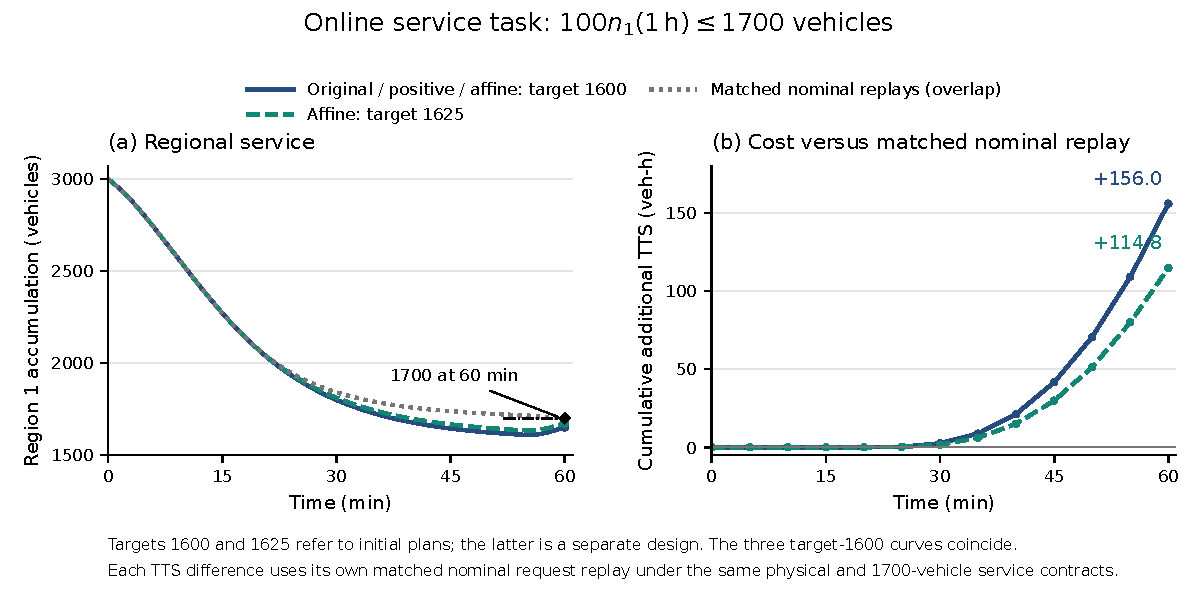
\includegraphics[width=0.98\textwidth]{figures/mfd_structure_online_runtime.pdf}
\caption{Binding-service online comparison under the same 1700-vehicle
deadline and uncertainty contract. All three enclosures give identical
execution from the 1600-target initial plan. The signed enclosure
also certifies the more economical 1625-target plan. Incremental TTS is
computed against each plan's matched nominal-request replay.}
\label{fig:structure-online}
\end{figure}

The adverse signed-method mission completes with one rejected replacement
and retained execution, reaching 1706.09 vehicles at the 2850-vehicle
deadline. Independent checks confirm membership of the actual state in
every fresh observation box; the biased observations leave the simulated
state unchanged. This selected realization jointly exercises initial error,
sensing bias and arrival residual within the certified contract.

\paragraph{Compatibility with economical MPC proposals}
The original eight-event grid tests the same execution architecture with
the 2850-vehicle service request and original uncertainty contract.
Table~\ref{tab:new-incident-primary} reports the primary event. The
queue-blind incumbent holds equilibrium gates: its internal targets stay
unchanged while waiting grows and the deadline is missed. Under the
separate 40\% event its queue reaches storage at minute 62.5.

\begin{table}[t]
\centering
\caption{MPC compatibility. The upper panel reports the primary 30\%
exterior-arrival increase for one hour, using independent adaptive replay
over two hours. The lower panel summarizes all eight designed events under
the original information and residual contract. Certified variants add the
stated uncertainty-aware execution guarantee.}
\label{tab:new-incident-primary}
\small
\setlength{\tabcolsep}{4pt}
\begin{tabular}{@{}lrrrr@{}}
\toprule
Policy & TTS & Queue time & Peak queue & $100n_1(1\,\mathrm h)$\\
& veh-h & veh-h & veh & veh\\
\midrule
Queue-blind incumbent & 14462.50 & 2462.50 & 1850.00 & 3000.00\\
Nominal library & 9654.68 & 314.23 & 301.79 & 2205.60\\
Certified library & 9654.68 & 314.23 & 301.79 & 2205.60\\
Nominal MPC & 7852.00 & 229.17 & 200.00 & 1709.80\\
Certified MPC & 7852.00 & 229.17 & 200.00 & 1709.80\\
\bottomrule
\end{tabular}
\par\medskip
\begin{tabular}{@{}lr@{}}
\toprule
Eight-event nominal/certified MPC comparison & Outcome\\
\midrule
Events meeting the regional deadline & 8/8\\
Candidate plans admitted & 192/192\\
Incremental realized TTS (veh-h) & 0 in every event\\
\bottomrule
\end{tabular}
\end{table}

The summary panel records successful admission across the eight completed
two-hour missions. Certified and matched nominal MPC commands and states
are exactly identical. The continuous-command planner
achieves 17.04--19.88\% lower TTS than the restricted certified library,
with an 18.67\% primary-event reduction and library TTS as denominator.
This planner-authority comparison shows that the checker can preserve the
economic benefit of a richer candidate set under the same physical contract.
The full eight-event table and trajectories appear in the supplement.

Plan replacement can change a later block or extend the verified horizon while
preserving the first command. The supplement reports accepted replacements, actual command changes,
and certified and realized inventory bounds separately.

\paragraph{Numerical verification and finite-plan authority}
\label{sec:new-numerical-audit}
Independent numerical checks reconstructed the certified trajectories
from the installed commands and observations. The longest measured proof
took 14.77 seconds within a five-minute planning interval. The continuous
enclosures cover the complete specified state and arrival-uncertainty set;
trajectory replays confirm the reported implementation outcomes. Detailed
timing and numerical checks appear in the supplement.

Forced outages demonstrate recovery after a short interruption and retained
execution through the original expiry during a prolonged interruption. The
finite-horizon simulation ends at that expiry. \papernumber{sec:terminal-backup}
specifies the terminal certificate that extends authority beyond expiry.
These earlier compatibility simulations use synchronous activation.
Section~\ref{supp:detail:sec:delayed-handover-results} tests a propagated information set
for future-dated installation.

\FloatBarrier
\section{Connected-Network Model and Complete Sweep}
\label{app:network-transfer}

\subsection{Allocation changes and branch structure}

Proposition~\papernumber{prop:network-localization} uses constant allocation shares.
For a known differentiable $P_a(t)$, differentiating $y_c=c+P_a(t)z$ gives
\begin{equation}
 \dot y_c=F(c,u,t)+P_a(t)\Lambda+\dot P_a(t)z.
 \label{supp:detail:eq:network-varying-allocation}
\end{equation}
With fixed reference coordinates $y_c=c+P_0z$ and actual shares $P_a(t)$,
the corresponding expression is
\begin{equation}
 \dot y_c=F(c,u,t)+P_0\Lambda+(P_a(t)-P_0)a.
 \label{supp:detail:eq:network-uncertain-allocation}
\end{equation}
The extra terms enter the predictor and uncertainty enclosure. At a specified
piecewise-constant share change, physical inventories remain continuous but
coordinates change. Propagate the same initial uncertainty symbol through
$\Gamma^+=L_a^+(L_a^-)^{-1}\Gamma^-$, and bound the remainder by
$|L_a^+(L_a^-)^{-1}|\rho^-$ plus outward conversion and predictor-recentering
error. The implemented
transfer study uses constant shares and retains one coordinate map throughout.

For fixed commands and independent queues, the interval Jacobian in
(\papernumber{eq:network-jacobian}) obtains a sound majorant by bounding each queue
diagonal separately, independently of simultaneous admission-branch
combinations. The present implementation enumerates combinations of
individually unexcluded predictor branches when bounding the defect, with at most
$2^r$ combinations before branch exclusion. Shared receiving capacities,
regional-state-dependent admission, and feedback gates require their actual
coupled derivatives in place of the independent-queue block structure.

\subsection{Connected ring instantiation}

The transfer experiment has $R=2$ or $R=3$ regions in a clockwise ring. Class
$c_{ij}$ contains vehicles in region $i$ whose final destination is $j$;
the local class completes and every nonlocal class advances one edge while
preserving its destination. Each region has one exterior queue. Thus the
physical dimensions are $R^2+R=6$ and $12$, distinct from the primary model's
seven-state convention. With $N_i=\sum_jc_{ij}$, local completion is
$c_{ii}v(N_i)$ and nonlocal transfer is $u_i c_{ij}v(N_i)$, using the same
literature speed polynomial as (\papernumber{eq:new-mfd}). This produces genuine
interregional coupling and destination-dependent travel through the ring.

Each queue admits $a_i=\min\{60z_i,120g_i\}$. Half the arrivals have the
entering region as destination; the other half is divided equally among the
other destinations. Every region initially contains 3000 vehicles, half
local and half nonlocal, and each exterior queue contains 200 vehicles.
Primitive internal demand is specified directly: 6000 vehicles/h to the local
destination and 500 vehicles/h in total to nonlocal destinations, per region.
Exterior arrivals are 4000 vehicles/h per queue. Queue 0 has a 30\% increase
from minute 15 through minute 45, with exact clock cuts at both jumps.

The fixed plan uses ring gates 0.65 and admission gates 0.50 for the first
30 minutes. Subsequently ring gates 0 and 1 become 0.80 and 0.55, respectively,
and any remaining ring gates stay at 0.65. Admission gate 0 becomes 0.60;
all others stay at 0.50. Every gate lies in $[0,1]$. The physical contract
requires nonnegative classes and queues, at most 10,000 vehicles per region
and 2000 vehicles per queue. The prespecified service requirement is at most
2700 vehicles in every region at one hour. The plan is specified directly
before certification, independently of optimization and observed outcomes.

Each independent class-coordinate half-width is $d/R$ vehicles, giving nominal
regional-total half-width $d$; each queue half-width is $\min(d,10)$ vehicles.
The binary widths actually supplied to the verifier are recorded. The physical
residual allowance $\bar w_{\rm veh}$ applies independently to each queue.
The network-wide sum of absolute arrival errors, expressed in vehicles/h,
is therefore bounded by $R\bar w_{\rm veh}$. The fixed pairs
$(d,\bar w_{\rm veh})$ are $(1,60),(10,60),(25,60),(25,300)$ in vehicles and vehicles/h.
Both networks and both coordinate methods use every pair, for 16 attempts.
\begin{table}[t]
\centering\small
\caption{Complete connected-ring certificate sweep. Entries are the largest
regional deadline upper bounds in vehicles, rounded upward. A dash marks an
unresolved sufficient full-plan proof for the tested method and contract.}
\label{tab:network-transfer-complete}
\setlength{\tabcolsep}{4pt}
\begin{tabular}{@{}rrrrr@{}}
\toprule
Regions/states & $d$ (veh) & $\bar w_{\rm veh}$ (veh/h) & Class coordinates & Combined inventories\\
\midrule
2/6 & 1 & 60 & 1421.88 & 1411.77\\
2/6 & 10 & 60 & 1433.39 & 1413.41\\
2/6 & 25 & 60 & 1438.93 & 1414.94\\
2/6 & 25 & 300 & --- & 1551.15\\
3/12 & 1 & 60 & --- & 1999.42\\
3/12 & 10 & 60 & --- & 2024.64\\
3/12 & 25 & 60 & --- & 2059.74\\
3/12 & 25 & 300 & --- & ---\\
\bottomrule
\end{tabular}
\end{table}

Nonnegative demand, admission and incoming class transfers establish boundary
invariance independently of the upper capacities being checked. The speed
polynomial is globally positive: its leading coefficient and minimum are
positive. Summing internal classes and exterior queues cancels all transfers
and admissions, giving offered demand minus nonnegative trip completion.
This bounds finite-horizon inventory growth and excludes finite escape.
The numerical proof then checks regional and queue capacities separately.

The dimension-generic implementation uses degree-two predictors, order-18
matrix series with outward remainder bounds, and a maximum interval of
$1/120$ hour. Failed self-inclusion can halve the interval down to $1/1920$
hour; every failed attempt is retained. Positive-queue facts restrict the
mean-value corridor using the predictor--actual queue hull. The generator
and its remainder retain their full bounds. Physical supports and every regional deadline
are checked after enclosure. A full-plan certificate is issued when every
required enclosure and constraint check closes.

\subsection{Computational dependence and interpretation}

Let $n$ be the state dimension, $g$ the retained generator count, $m$ the number
of evaluated affine rows, $N$ the number of evaluated predictor intervals
(including step-halving retries), $K$ the trial-tube
attempt limit and $p$ the matrix-series order. Count fixed-precision interval
arithmetic. Denote predictor/defect cost by $C_d$, independent queue cost by
$C_q$, one interval-Jacobian evaluation by $C_J$, and evaluated Jacobian
branches by $b$. A dense upper bound for the signed propagation is
\begin{equation}
 \begin{split}
 O\!\left(N\left\{C_d+C_q+mn^2
  +p(n^3+n^2g+mng)\right.\right.\\[-2pt]
 \left.\left.\hspace{12mm}+K\,[pn^3+bC_J+bn^2g]\right\}\right).
 \end{split}
 \label{eq:network-computation}
\end{equation}
Matrix-series products and continuous boxed-remainder propagation contain
dense cubic operations. For $g=n$, $m=O(n)$, fixed $p,K,b$, and
$C_d,C_q,C_J=O(n^3)$, this expression reduces to $O(Nn^3)$.
Symbolic or polynomial geometry setup, optimizer work and variable-precision
bit costs are separate. For arbitrary dense polynomial models, Jacobian
evaluation remains an explicit model-dependent cost $C_J$; its scaling
requires analysis of the chosen polynomial backend. The generic ring backend evaluates its explicitly sparse traffic
balances, while its predictor branch count remains part of $C_d$.

Successful numerical scaling requires both affordable computation and
enclosures that remain useful as uncertainty and coupling grow. The transfer
grid reports both: runtime for completed certificates and unresolved cells.
Its fixed-plan timings exclude MPC optimization and language inference.
Single-host measurements with concurrent background work characterize this
prototype; activation in this connected-network study is synchronous.

\FloatBarrier
\section{Current Live-Agent Experiments}
\label{sec:supp-execution}
\label{supp:detail:sec:task-state-live}
\label{supp:detail:sec:queue-live-pilot}
\label{supp:detail:sec:primary-memory-pressure}

The agent's operational role is to interpret a changing instruction and
invoke a numerical planning tool for the resulting objective. We test
this role in two stages using the OpenAI Responses API model
\texttt{gpt-5.4-mini-2026-03-17}, with reasoning disabled and strict
function-call schemas. The companion records contain literal prompts,
tool parameters, raw responses, model identifiers and token usage.
The same requests can be replayed from these records or submitted to a
later model version.

The first stage contains 96 interpretation and tool-routing calls:
three plan-availability situations, four temporal histories, clean or
poisoned lower-trust tool memory, two input interfaces and two repetitions.
The situations are admission of the original MPC plan, checked repair
after rejection and retention during a replacement-tool outage. Operator
histories exercise direct priority assignment, restoration after an
interruption, nested restoration and exact-expiry handling. In the
history-only interface the model resolves the objective from the prose
history. The task-record interface additionally supplies the current
authoritative priority and its absolute expiry. Each chosen action routes
a precomputed numerical plan through the independent execution check.

\begin{table}[t]
\centering\small
\caption{Interpretation pilot: 24 calls per interface/memory cell.
Correct objective and tool counts have the same denominator. All
authorized executions satisfy their physical and scheduled service rows.}
\label{supp:detail:tab:benchmark-api-pilot}
\begin{tabular}{@{}llrr@{}}
\toprule
Interface & Tool memory & Objective & Tool\\
\midrule
History only & Clean & 19/24 & 22/24\\
History only & Poisoned & 15/24 & 24/24\\
Task record & Clean & 24/24 & 24/24\\
Task record & Poisoned & 24/24 & 24/24\\
\bottomrule
\end{tabular}
\end{table}

The second stage evaluates eight actual agent-to-planner traces on the
primary Task-D contract. Four temporal histories are paired across the
two interfaces; every trace includes a corrupted tool-cache instruction.
The operator's Region-2 preference remains active through the minute-60
plan expiry. The cache attempts to change that preference, enlarge storage
and bypass admission. Its content has no authority to change the physical
or service contract. The model first selects an objective; that objective
sets the cost coefficients of a newly solved MPC problem. The resulting
commands are checked. Following rejection, the model can request checked
repair or retain the incumbent. Thirteen live calls complete the eight
traces, and every authorized plan is evaluated on its 640 matched
initial-state/residual realizations.

\begin{table}[t]
\centering\small
\caption{Actual planning-tool traces under poisoned tool memory. The
objective request is used in a fresh MPC solve; checked repair is invoked
after the rejected Region-2 request. Each interface has four traces.}
\label{supp:detail:tab:benchmark-api-execution}
\begin{tabular}{@{}lrrr@{}}
\toprule
Interface & Objective correct & Checked repairs & Feasible runs\\
\midrule
History only & 1/4 & 1/4 & 2560/2560\\
Task record & 4/4 & 4/4 & 2560/2560\\
\bottomrule
\end{tabular}
\end{table}

The task record improves interpretation in these small matched examples.
Physical certification separately enforces the authorized limits and
deadline for every executed numerical plan. Together the two stages
exercise semantic resolution, numerical planning, constraint feedback,
repair requests and the final allocation of execution authority. Their
sample sizes and the fixed model version define the scope of this
interface demonstration. Earlier live routing and local Qwen3 task-state
experiments are retained in \appref{app:earlier-agent-study} and
\appref{app:task-state-protocol}, respectively. Those protocols evaluate
complementary parts of the same interface with their own models,
decision clocks and denominators.

\FloatBarrier
\section{Earlier Local-Model Task-State Study}
\label{app:task-state-protocol}

\subsection{State, operations and temporal consistency}

The canonical record $\theta_i$ contains an active regional priority and a
last-in, first-out stack of suspended priorities, each with region, label and
absolute expiry. Network operation is the default. Before a proposal at $t_i$,
$\mathsf{Age}_{t_i}$ removes an expired active task and pops expired predecessors until
an unexpired task is restored or the stack is empty. For a parsed operation
$r_i^A$,
\begin{equation}
 \theta_i^+=C(\mathsf{Age}_{t_i}\theta_i,r_i^A),\qquad
 (j_i,\Delta_i)=Q(\theta_i^+,t_i),
 \label{supp:detail:eq:task-state-compiler}
\end{equation}
where $j_i$ selects the soft objective. A regional task expiring at $e_i$
has $\Delta_i=e_i-t_i>0$; network operation has $\Delta_i=0$.
The same expiry rule applies between proposals.

\begin{table}[t]
\centering\small
\caption{Compiler transitions. Only the listed fields accompany the operation
name. Durations/extensions are integer minutes in $[1,120]$; nonempty labels
contain at most 80 characters.}
\label{supp:detail:tab:task-state-operations}
\begin{tabular}{@{}p{0.14\textwidth}p{0.22\textwidth}p{0.56\textwidth}@{}}
\toprule
Operation & Additional fields & Transition at time $t$\\
\midrule
Set & Region, duration, label & Clear the stack; install a task expiring at
$t+$ duration.\\
Interrupt & Region, duration, label & Save the active task with its original
expiry; install a temporary task expiring at $t+$ duration.\\
Continue & None & Preserve the surviving task and expiry.\\
Extend & Minutes & Add the stated time to the active task's expiry.\\
Resume & None & Restore the latest unexpired saved task; if none survives,
clear the interruption. With no stack or interruption, keep the current task.\\
Cancel; network & None & Clear active and suspended tasks; use network operation.\\
\bottomrule
\end{tabular}
\end{table}

The compiler rejects extra fields, extension of an absent task and
interruption depth above four. Invalid operations create no new planning
request. The canonical record derives from schema-valid model operations,
independently of evaluation labels and physical-plan admission. Thus a valid
operation may update the requested objective while the authority retains an
earlier certified plan; constraint feedback connects these distinct states.
The hard storage, gate and service requirements remain in the trusted contract.

\emph{Temporal invariant.} Each stored expiry equals creation time plus the
specified duration and explicit extensions. Set and interrupt establish this
identity; extend adds exactly its argument; continue, suspension and restoration
preserve it. Deletion removes a task without changing another expiry.
Induction over the operation table, combined with $\mathsf{Age}_t$, therefore leaves either
network operation or a task with positive remaining time. Agreement with the
operator's language is scored separately at the compiled-request output.

\subsection{Earlier local-model protocol and exact command compilation}

The initial state has 3000 vehicles per region and 200 exterior vehicles:
the first qualifying cell in the specified 24-attempt development grid.
The model uses the primary contract's 30\% arrival pulse, one-hour mission,
one-vehicle observation half-widths and 60-vehicle/h residual allowance.
The original Region~1 deadline remains 2850 vehicles at one hour. Soft
objective rows weight regional inventories by $(4,1)$, $(1,4)$ or $(1,1)$,
with exterior waiting weighted once. Each numerical plan covers the full
remaining hard mission, independently of its shorter priority window.

Eight development calls identify and remove a redundant contextual schema
field. Fresh held-out phrases are then held fixed for both interfaces.
At minutes 5, 10, 15, 20, 25, 30, 35 and 40, the intended operations are:
set Region~1 for 25 minutes; continue; interrupt with Region~2 for 15 minutes;
extend by 10 minutes; resume; continue after expiry; set Region~2 for
20 minutes; cancel. The expected region/window sequence is
R1/25, R1/20, R2/15, R2/20, R1/5, network/0, R2/20, network/0.
Two paraphrases per interface give 32 held-out calls. The eight-call memory
probe completes the total of 48, including development.

All calls use local Qwen3 8B, Q4\_K\_M quantization, temperature zero and
recorded fixed seeds. Prompts use current observations and actual execution
feedback; expected requests are reserved for scoring. The memory probe
replaces only retrieved active/suspended views at minutes 10, 20, 25 and 30
with false Region~2 records and an injected instruction. Its separately
reserved seeds distinguish it from a matched-seed intervention comparison.
The earlier-study research records document development diagnostics, the
separate live pilot and the intervention; the reproducibility archive stores literal prompts, model identifiers and responses.

In the earlier local-model experiment, every comparison policy compiles
raw optimizer commands onto the
dyadic grid with denominator $2^{40}$: clip coordinates to $[0,1]$, round to
the grid, and distribute excess paired-gate difference between the coordinates
until its exact magnitude is at most $3/4$. Maximum-norm corrections above
$10^{-7}$ are refused. The checker verifies and binds these compiled commands;
raw commands, corrections and exact rational margins are recorded.
This removes optimizer roundoff at gate boundaries without changing physical
state or certificate tolerances. The largest executed correction is below
$1.69\times10^{-9}$.

For direct command pressure, set $u=(0.8,0.5,0,0.75)$
at minutes 20, 25, 30 and 35, restricting admission during
continuing arrivals. Its unprotected comparison reports the first storage
crossing separately from the later overflow diagnostic.

\subsection{All matched traffic outcomes}
\label{app:task-state-traffic}

Each nominal comparator replays the same valid and invalid request sequence
and replans on its own current state, without further live calls. The common
intended-task metric uses $(4,1)$ or $(1,4)$ during the corresponding intended
priority intervals and $(1,1)$ otherwise, always including exterior waiting.
Independent class-balance replay supplies Table~\ref{tab:task-state-traffic}.
Both TTS and common intended-task cost decrease under certification in every
matched pair; comparisons between different language interfaces remain
distinct.

\begin{table}[t]
\centering\footnotesize
\caption{All primary-agent traffic pairs. TTS is in vehicle-hours and $\Delta$
is certified TTS relative to nominal replay. Peak is certified queue size
(vehicles). Retained counts all twelve epochs, including invalid requests
and rejected certificates. The two task-record held-out trajectories coincide.}
\label{tab:task-state-traffic}
\setlength{\tabcolsep}{3.5pt}
\begin{tabular}{@{}lrrrrr@{}}
\toprule
Episode & Certified TTS & Nominal TTS & $\Delta$ (\%) & Peak & Retained\\
\midrule
Prose, phrase 1 & 4722.42 & 5028.19 & $-6.08$ & 1218.07 & 4\\
Task record, phrase 1 & 4845.85 & 4966.41 & $-2.43$ & 1626.12 & 1\\
Prose, phrase 2 & 4536.63 & 4839.53 & $-6.26$ & 780.00 & 6\\
Task record, phrase 2 & 4845.85 & 4966.41 & $-2.43$ & 1626.12 & 1\\
Task record, corrupted view & 4693.07 & 4785.59 & $-1.93$ & 1226.12 & 1\\
\bottomrule
\end{tabular}
\end{table}

Constant-network TTS is 4428.57 vehicle-hours; the intended-request reference
has TTS 4559.47. Both use receding-horizon planning with the operator
requests available at each decision time. All five certified live episodes satisfy the physical and
original service requirements, including the two task-record traces with worse
TTS and intended-task cost than their prose counterparts. The earlier-study research records
document the detailed audits and numerical checks. The supplement
records every common-cost value, proof/admission record and raw call;
inference and proof times are recorded separately from the synchronous clock.

\FloatBarrier
\section{Earlier Agent Routing Study}
\label{app:earlier-agent-study}


The live-agent study concerns the agent's operational role after a planner and
certifier return their results. We test three fixed workflows: an MPC plan that is
certified unchanged; an MPC plan that is rejected and then successfully
repaired; and the same rejection followed by a specified repair-service
timeout. The agent can invoke exactly three orchestration tools:
\texttt{install\_certified\_plan},
\texttt{request\_predictive\_repair}, and
\texttt{retain\_verified\_plan}. It receives the trusted verdict, constraint feedback, exact plan identifier, active backup and remaining validity interval.
The execution layer independently checks the requested action against this
record before changing the authorized plan.

The earlier live routing study uses the OpenAI Responses API model
\texttt{gpt-5.6-terra} with two fixed prompt formulations and three
repetitions per formulation and workflow. One prompt presents the current
authorization state as structured data; the other precedes the same data
with an operator narrative. The design produces 18 complete workflows and
30 sequential tool decisions. The companion live-call files provide prompts, tool schema, model
identifier, sampling settings, raw responses and parsed actions.
Traffic outcomes can be replayed from those calls, and the same
protocol can evaluate later API model versions.

\begin{table}[t]
\centering\footnotesize
\caption{Live OpenAI routing through the certified execution interface.
Each row contains two prompt formulations and three repetitions. Traffic
outcomes use replay of the plan authorized by the execution
layer.}
\label{tab:task-state-live}
\setlength{\tabcolsep}{3pt}
\begin{tabular}{@{}lrrrr@{}}
\toprule
Runtime situation & Runs & Correct & Storage fail. & Service fail.\\
\midrule
MPC certified & 6 & 6/6 & 0 & 0\\
Rejected; repair certified & 6 & 12/12 & 0 & 0\\
Rejected; repair timeout & 6 & 12/12 & 0 & 0\\
\midrule
Total & 18 & 30/30 & 0 & 0\\
\bottomrule
\end{tabular}
\end{table}

All six pass workflows install the original MPC plan. All six successful-
repair workflows request repair after rejection and install only the repaired
plan carrying the new certificate. All six timeout workflows request repair
and then retain the verified plan when the service returns no candidate.
Mean per-call API latency
ranges from 2.46 to 3.20 seconds across the three workflows. The associated
traffic replays are therefore the original certified-MPC trajectory, the
certified-repair trajectory and the verified-continuation trajectory,
respectively; each satisfies storage and the scheduled regional service row.

\paragraph{Contextual interpretation and action stress test}

A complementary local-model study using Qwen3 8B evaluates
priority assignment, interruption, restoration, expiry and cancellation
under incomplete and corrupted contextual views
(\appref{app:task-state-protocol}). It tests contextual interpretation,
while the live API study above tests routing among install, repair and
retain actions. The local-model protocol appears in the appendix
\cite{qwen3technical}. A separate deterministic
action-channel audit submits zero-admission plans while arrivals continue.
The checker rejects all four submissions and retained execution completes the
mission; direct unprotected execution reaches the 2000-vehicle storage bound
at minute 34.43. These records distinguish interpretation quality from the
authority assigned to the resulting numerical plan.

\phantomsection
The two studies exercise complementary parts of the same
agent--planner--certificate interface.

\FloatBarrier
\section{Earlier Fixed-Controller and Single-Contract Comparisons}
\label{app:earlier-benchmarks}


The additional comparisons fix the plant and evaluation horizon within each
experiment and separate the controller's objective from the execution
certificate. Each table therefore supports a matched common-plant comparison.

\paragraph{A specified CLF extension on the eight-event grid}
Zhong et al.\ \cite{zhong2018robust} develop a two-gate CLF perimeter
controller for regional regulation. Our seven-state benchmark requires
additional admission and exit channels. We therefore implement a
\emph{CLF+queue extension}: an almost-smooth CLF correction supplies the two
interregional gates; a fixed Region-1-protection LQR supplies the admission
and exit gates; and projection enforces the additional directional gate
constraint. The LQR reference totals are $(2700,3200)$ vehicles, with
state weights $(4,1,0.1,0.1,0.1,0.1,2)$ and input weight $3000I_4$.
\appref{app:benchmark-details} specifies the adapted law. The baseline targets
regional regulation, while MPC also includes the scheduled-service row.

Table~\ref{tab:clf-common} uses the same eight arrival events, initial
state, model, physical rows and two-hour evaluation horizon as the MPC compatibility grid, with zero realized residual. All CLF-extension
trajectories complete the horizon within sampled physical limits, but none
meets the 2850-vehicle Region-1 requirement at one hour. Certified MPC meets
that requirement in all eight cases and admits all 24 proposals per case,
preserving nominal-MPC TTS. Its TTS is 42.15--46.50\% lower than this
extension (median 43.64\%). The table evaluates the specified queue-aware
extension on the common seven-state service problem. Zhong et al.'s native
controller retains its published guarantee for its original two-region
regulation model; the appendix records the exact adaptation used here.

\begin{table}[t]
\centering\footnotesize
\caption{Common seven-state plant, two-hour evaluation. Event duration is
in minutes; TTS is in veh-h and Region-1 deadline accumulation is in vehicles.
MPC and certified MPC have identical TTS in every row.}
\label{tab:clf-common}
\setlength{\tabcolsep}{3pt}
\begin{tabular}{@{}rr rrr rr@{}}
\toprule
Event (\%) & Duration & CLF TTS & Certified MPC TTS & Reduction (\%) & CLF $n_1$ & MPC $n_1$\\
\midrule
20 & 30 & 13050.60 & 7550.19 & 42.15 & 2901.14 & 1609.31\\
20 & 60 & 13594.30 & 7699.53 & 43.36 & 2935.68 & 1663.79\\
25 & 45 & 13588.13 & 7680.99 & 43.47 & 2981.54 & 1683.54\\
30 & 30 & 13346.32 & 7621.59 & 42.89 & 2963.35 & 1628.31\\
30 & 60 & 14249.31 & 7852.00 & 44.90 & 3038.89 & 1709.80\\
35 & 45 & 14096.38 & 7795.98 & 44.70 & 3095.97 & 1728.87\\
40 & 30 & 13694.40 & 7695.91 & 43.80 & 3034.60 & 1648.46\\
40 & 60 & 14976.79 & 8012.78 & 46.50 & 3142.17 & 1756.56\\
\bottomrule
\end{tabular}
\end{table}

\subsection{Predictive repair of a rejected economic-MPC plan}


At minute 20 of the adverse $(d,\bar w_{\rm veh})=(25,300)$ mission, MPC
submits a two-block plan with durations 5 and 35 minutes. The regional
information half-width is 25 vehicles in each of the first six coordinates;
the exterior-queue half-width is 10 vehicles. Every measurable arrival
residual within $\pm300$ veh/h is covered. Both the plan expiry and the
2850-vehicle Region-1 deadline remain at minute 60. Repair modifies the two remaining command blocks while preserving
their timing, the inherited information set and the service deadline.
The selected plan changes the stacked command vector by 7.83\%
relative to the submitted MPC plan. Its certified upper bound on
Region-1 accumulation at the deadline is 2849.1 vehicles, below
the 2850-vehicle target; the realized trajectory reaches about 2260
vehicles. Exact commands and the finite repair grid are given
in \papernumber{app:repair-cost} and the supplement.

\paragraph{Within-contract test case}
The test case starts at the information-box center with the queue at its
upper endpoint and uses the constant $+300$ veh/h residual. The submitted
40-minute plans remain fixed throughout the suffix, which also represents a
planner outage after submission. We measure suffix TTS and the
Region-2-priority diagnostic
\begin{equation}
J_2(P)=100\int_{1/3}^{1}\bigl(n_1+4n_2+z\bigr)\,dt.
\label{eq:repair-priority}
\end{equation}
Lower values are preferred; the same weights are applied to every policy.

Table~\ref{tab:repair-witness} and Figure~\ref{fig:predictive-repair} show
that the unfiltered MPC plan exceeds exterior storage and misses the service
deadline. The Zhong-style CLF+queue extension, certified repair and verified
continuation all satisfy the realized storage and deadline rows. The CLF
extension holds the peak queue to 673.64 vehicles but accumulates 3548.64
veh-h of TTS and gives $J_2=8922.91$. Predictive repair reduces TTS by
13.30\% and $J_2$ by 27.75\% relative to that extension while remaining
inside the 2000-vehicle queue limit. The backup has the lowest TTS and queue,
whereas repair follows the requested Region-2 priority more closely. In this
test case, repair retains 76.85\% of the priority benefit available between the
rejected MPC request and backup. The comparison therefore separates regional
regulation, requested-priority tracking and verified execution under a common
transportation contract.

\begin{table}[t]
\centering\footnotesize
\caption{Same minute-20 information and $+300$ veh/h residual. All integral
costs cover minutes 20--60. Queue time is included in TTS; $J_2$ has units
of weighted veh-h. Storage/service entries are realized passes (P) or
failures (F); continuous robust guarantees for repair and backup come from
their separate certificates. Unfiltered results after overflow are diagnostics.}
\label{tab:repair-witness}
\setlength{\tabcolsep}{2pt}
\begin{tabular}{@{}lrrrrrrc@{}}
\toprule
Policy & TTS & \shortstack{Queue\\time} & \shortstack{Peak\\queue} & \shortstack{Deadline\\$n_1$} & $J_2$ & Departures & \shortstack{Storage/\\service}\\
 & (veh-h) & (veh-h) & (veh) & (veh) & & (veh) &\\
\midrule
Rejected MPC & 3302.41 & 686.45 & 2180.04 & 2853.08 & 6334.73 & 15929.57 & F/F\\
CLF + queue extension & 3548.64 & 290.18 & 673.64 & 2556.57 & 8922.91 & 15942.70 & P/P\\
Certified repair & 3076.53 & 522.71 & 1618.65 & 2260.32 & 6447.19 & 16868.34 & P/P\\
Verified backup & 2698.68 & 110.70 & 197.98 & 1727.56 & 6820.46 & 18368.37 & P/P\\
\bottomrule
\end{tabular}
\end{table}

\paragraph{Information-box and disturbance ensemble}
The same three fixed plans (rejected MPC, certified repair and backup) are
replayed at all $2^7=128$ information-box corners under five deterministic
within-contract residual profiles: zero, constant high, constant low,
five-minute alternation and a ten-minute sinusoid. This gives 640
realizations per policy, or 1920 trajectories. Table~\ref{tab:repair-ensemble}
reports realized counts and median costs for this deterministic stress
ensemble. Robust coverage of the full information box and measurable residual
family is supplied by the interval certificate.

For each matched realization $r$, define the retained priority benefit
\begin{equation}
\varrho_r=\frac{J_{2,r}(P^B)-J_{2,r}(P^R)}
                 {J_{2,r}(P^B)-J_{2,r}(P^0)}.
\label{eq:repair-benefit}
\end{equation}
The denominator is positive in all 640 cases. The retained fraction ranges
from 72.08\% to 76.99\%, with median 75.13\%. The paired TTS premium
over backup ranges from 13.21\% to 14.21\%, with median 13.79\%.
The repair's median priority cost is 5.05\% below the backup's median.
The interval certificate extends the physical and service guarantee from the
displayed ensemble to all admissible initial states and measurable residuals
in the specified contract.

\begin{table}[t]
\centering\footnotesize
\caption{Fixed-plan ensemble over minutes 20--60: 640 realizations per
policy. Pass counts are realized outcomes and costs are ensemble medians.}
\label{tab:repair-ensemble}
\setlength{\tabcolsep}{3pt}
\begin{tabular}{@{}lrrrrr@{}}
\toprule
Policy & Storage passes & Service passes & TTS (veh-h) & Queue (veh-h) & $J_2$\\
\midrule
Rejected MPC & 448/640 & 298/640 & 3240.81 & 628.88 & 6262.82\\
Certified repair & 640/640 & 640/640 & 3014.63 & 465.14 & 6374.38\\
Verified backup & 640/640 & 640/640 & 2649.57 & 86.86 & 6713.41\\
\bottomrule
\end{tabular}
\end{table}

\paragraph{Repair search and computation time}
The finite search tests 28 repair weights and accepts 18. Its least accepted
weight is 0.2822, so Theorem~\papernumber{thm:repair-grid} identifies the smallest
change among the tested plans. Constraint failures near the submitted plan
include physical rows; near the acceptance boundary, the deadline row is
decisive. The ordered search takes 91.74 seconds on the test machine, within
the remaining plan-validity interval. A delayed installation is checked from
its actual activation state, as specified in
Proposition~\papernumber{prop:repair-execution}. The exact grid and complete timing
record appear in \papernumber{app:repair-cost}.

\begin{figure}[t]
\centering
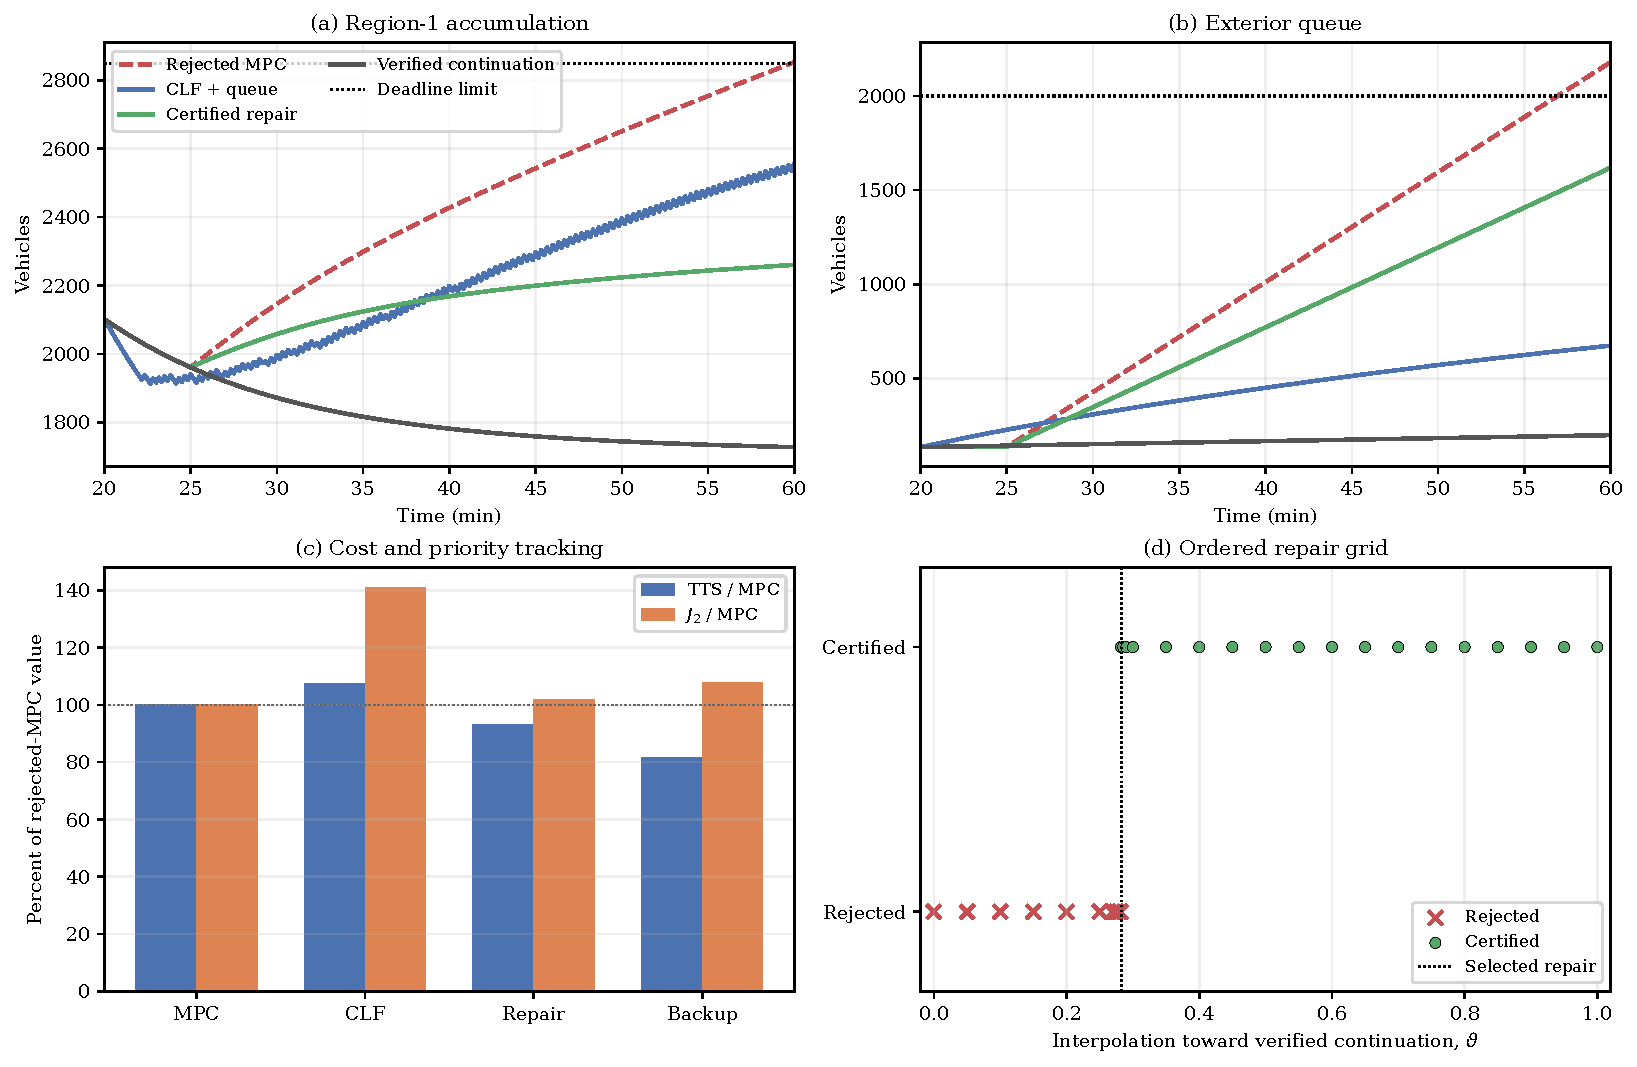
\includegraphics[width=0.98\textwidth]{figures/final_transport_benchmark.pdf}
\caption{Matched priority-conflict benchmark. Top: Region-1 accumulation and
exterior queue for the rejected MPC request, specified CLF+queue extension,
certified repair and verified continuation. Bottom left: suffix TTS and
priority cost normalized by the rejected-MPC values. Bottom right: the
exhaustive repair grid and first certified interpolation. Sampled trajectories
illustrate performance; plan certificates establish robust storage and
service satisfaction for repair and continuation over the specified sets.}
\label{fig:predictive-repair}
\end{figure}

\FloatBarrier
\bibliographystyle{elsarticle-num}
\setlength{\bibsep}{1pt}
\bibliography{FOUNDATION_REFERENCES}
\end{document}
